\chapter{Event Selection}

This Chapter outlines the event selection that we use for the analysis.  A list and brief description is given of both the data and the Monte Carlo generated events. Also the cuts and motivation for the analysis preselection is given.

\section{Datasets}

The focus of this analysis is on a massive Higgs boson which is above the ZZ production threshold of 200 GeV.  Because of this high energy, the decay of one of the Z bosons will produce a pair of high $p_T$ leptons.  This will primarily fire the double-lepton HLT paths and be stored in one of the two primary datasets: DoubleElectron or DoubleMuon.  For 2012 we are using the double lepton primary datasets corresponding to 19.6 $fb^{-1}$ at 8 TeV. The data samples for 2012 are listed in Appendix~\ref{sec:tablessamples}.  Each block of data undergoes data quality monitoring (DQM) both in real-time and after the data is recorded.  Only the data recorded under good conditions for each sub-detector is certified.  Subsequently, only data that is certified as good is used in this analysis. This analysis is done on the 2012 datasets but is combined with the previous results (2011) at the end.

The data that is used in this analysis is run over centrally produced datasets that are called primary datasets.  Primary datasets are filled with events that pass the high-level triggers that are identified with that dataset.  The three primary datasets that we are concerned with are the DoubleMu, DoubleElectron, and MuEG.  The DoubleMu must have two muons that fire a specific muon HLT, DoubleElectron must fire two specific electron HLT, and MuEG must have an electron and muon that fire one of the MuEG HLTs.  More details will be given later in this chapter.



%\begin{table}[htb]
%\caption{%
%  2012 data samples.
%}
%\begin{center}
%  \begin{tabular}{ | c | c | c |} \hline
%    Channel & Dataset Name & Luminosity [$pb^{-1}$] \\ \hline \hline
%    $2\Pgm 2\Pq$ & /DoubleMu/Run2012A-13Jul2012-v1/AOD & 808 \\ 
%    & /DoubleMu/Run2012A-recover-06Aug2012-v1 & 82 \\ 
%    & /DoubleMu/Run2012B-13Jul2012-v4/AOD & 4429 \\ 
%    & /DoubleMu/Run2012C-24Aug2012-v1/AOD & 495 \\ 
%    & /DoubleMu/Run2012C-PromptReco-v2/AOD & 6394 \\ 
%    & /DoubleMu/Run2012D-PromptReco-v1/AOD & 4580 \\ \hline
    
%    $2\Pe 2\Pq$ & /DoubleElectron/Run2012A-13Jul2012-v1/AOD & 808 \\ 
%    & /DoubleElectron/Run2012A-recover-06Aug2012-v1 & 82 \\
%    & /DoubleElectron/Run2012B-13Jul2012-v4/AOD & 4429 \\ 
%    & /DoubleElectron/Run2012C-24Aug2012-v1/AOD & 495 \\ 
%    & /DoubleElectron/Run2012C-PromptReco-v2/AOD & 6394 \\ 
%    & /DoubleElectron/Run2012D-PromptReco-v1/AOD & 4580 \\ \hline

%    $\Pgm \Pe \Pq \Pq $ & /MuEG/Run2012A-13Jul2012-v1/AOD & 808 \\ 
%    & /MuEG/Run2012A-recover-06Aug2012-v1/AOD & 82 \\ 
%    & /MuEG/Run2012B-13Jul2012-v4/AOD & 4429  \\
%    & /MuEG/Run2012C-24Aug2012-v1/AOD & 495  \\ 
%    & /MuEG/Run2012C-EcalRecover 11Dec2012-v1/AOD & 134  \\
%    & /MuEG/Run2012C-PromptReco-v2/AOD & 6394 \\
%    & /MuEG/Run2012D-PromptReco-v1/AOD & 7274 \\ \hline
    %\multicolumn{2}{|c|}{Photon purity cuts} \\ \hline
%  \end{tabular}
%\end{center}
%\label{tab:2012datasamples}
%\end{table}




\subsection{Simulated Events}

Monte Carlo (MC) simulations are useful for studying the properties of the SM Higgs boson and the backgrounds that are relevant to this analysis.  The dominant background in this analysis is the inclusive Z production with jets. Particularly those jets coming from b-quarks.  The Z+Jets sample uses the MADGRAPH generator~\cite{MadGraph07}. MADGRAPH is a Next-to-Leading-Order (NLO) matrix element generator.  Other backgrounds are $\Pqt \Paqt$, ZZ, WW and WZ.  The main portion of the top background is from $\Pqt \Paqt \rightarrow 2l2\nu 2b$ and the sample for this is generated using POWHEG~\cite{Powheg04,Powheg07,Powheg08} which is interfaced with PYTHIA 6~\cite{pythia} to do the final parton showering and hadronization.  For ZZ, WZ, and WW, they are fully generated with PYTHIA 6.  The Monte Carlo samples for these processes are listed in Appendix~\ref{sec:tablessamples}. 

The signal Monte Carlo samples used in this analysis were generated using POWHEG and vary for $M_H$ from 230 $GeV/c^2$ up to 1000 $GeV/c^2$.  These samples can also be seen in Appendix~\ref{sec:tablessamples}.  Each sample has 3$\times 10^{-5}$ events. The cross-sections multiplied by the branching ratio for $H \rightarrow ZZ \rightarrow 2l2q$ are listed as well.  The $H \rightarrow ZZ$ branching fraction is provided as a function of the Higgs boson mass by the LHC Higgs cross section working group~\cite{LHCHiggsCrossSectionWorkingGroup:2011ti,LHCHiggsCrossSectionWorkingGroup:2012ti}. The branching ratios of $Z \rightarrow \Plp \Plm$ and $Z \rightarrow \Pq \Paq$ are from the Particle Data Group (PDG)~\cite{pdg}. These numbers can be found in Appendix~\ref{sec:tablessamples}.

%\begin{table}[htb]
%\caption{%
%  2012 background MC samples.
%}
%\footnotesize
%\begin{center}
%  \begin{tabular}{ | c | c | c | c |} \hline
%    Process & Dataset Name &  $\sigma$ [pb] &  Luminosity [$fb^{-1}$] \\ \hline \hline
%    Z+jets (inclusive) & DYJetsToLL\_M-50\_TuneZ2Star\_8TeV-madgraph	& 3503.71 & 8.7 \\ 
%    & & & \\
%    
%    Z+1 jet (exclusive) & DY1JetsToLL\_M-50\_TuneZ2Star\_8TeV-madgraph	& 660.6 & 36.4 \\ 
%    Z+2 jet (exclusive) & DY2JetsToLL\_M-50\_TuneZ2Star\_8TeV-madgraph	& 215.1 & 101.6 \\ 
%    Z+3 jet (exclusive) & DY3JetsToLL\_M-50\_TuneZ2Star\_8TeV-madgraph	& 65.79 & 167.4 \\ 
%    Z+4 jet (exclusive) & DY4JetsToLL\_M-50\_TuneZ2Star\_8TeV-madgraph	& 27.59 & 232.1 \\
%    & & & \\
%    $\Pqt \Paqt$ & TTJets\_TuneZ2star\_8TeV-madgraph-tauola	& 23.38 & 461 \\ 
%    WW & WW\_TuneZ2star\_8TeV\_pythia6\_tauola	&	57.1097 & 168 \\ 
%    WZ & WZ\_TuneZ2star\_8TeV\_pythia6\_tauola	&	22.88 & 424  \\ 
%    ZZ & ZZ\_TuneZ2star\_8TeV\_pythia6\_tauola	&	17.654 & 549 \\ \hline
%    %\multicolumn{2}{|c|}{Photon purity cuts} \\ \hline
%  \end{tabular}
%\end{center}
%\label{tab:2012backmcsamples}
%\end{table}
%\normalsize


%%%%%%%%%%%%%%%%%%%%%%%%%%%%%%%%%%%%%%%%%%%%%%%%%
%\begin{table}[htb]
%\caption{
%POWHEG signal MC samples $H \rightarrow ZZ \rightarrow 2l2q, \,\,\,\, l = e, \mu, \tau$ 2012.
%}
%\label{tab:2012sigmcsamples}
%\vspace*{\medskipamount}
%\begin{center}
%\scriptsize
%\begin{tabular}{|c|l|c|}
%\hline
%$M_H$ (GeV) & Name & $\sigma(H \rightarrow 2l2q)$ [pb]  \\ \hline \hline
%200 & /GluGluToHToZZTo2L2Q\_M-200\_8TeV-powheg-pythia6/ & 0.2566 \\ & Summer12-PU\_S7\_START52\_V9-v1/AODSIM &  \\ \hline
%210 & /GluGluToHToZZTo2L2Q\_M-210\_8TeV-powheg-pythia6/ & 0.2538 \\ & Summer12-PU\_S7\_START52\_V9-v1/AODSIM &  \\ \hline
%220 & /GluGluToHToZZTo2L2Q\_M-220\_8TeV-powheg-pythia6/ & 0.2416 \\ & Summer12-PU\_S7\_START52\_V9-v1/AODSIM &  \\ \hline
%230 & /GluGluToHToZZTo2L2Q\_M-230\_8TeV-powheg-pythia6/ & 0.2278 \\ & Summer12-PU\_S7\_START52\_V9-v1/AODSIM &  \\ \hline
%250 & /GluGluToHToZZTo2L2Q\_M-250\_8TeV-powheg-pythia6/ & 0.2022 \\ & Summer12-PU\_S7\_START52\_V9-v1/AODSIM &  \\ \hline
%275 & /GluGluToHToZZTo2L2Q\_M-275\_8TeV-powheg-pythia6/ & 0.1751 \\ & Summer12-PU\_S7\_START52\_V9-v1/AODSIM &  \\ \hline
%300 & /GluGluToHToZZTo2L2Q\_M-300\_8TeV-powheg-pythia6/ & 0.1563 \\ & Summer12-PU\_S7\_START52\_V9-v1/AODSIM &   \\ \hline
%325 & /GluGluToHToZZTo2L2Q\_M-325\_8TeV-powheg-pythia6/ &  0.1478 \\ & Summer12-PU\_S7\_START52\_V9-v1/AODSIM &   \\ \hline
%350 & /GluGluToHToZZTo2L2Q\_M-350\_8TeV-powheg-pythia6/ & 0.1482 \\  & Summer12-PU\_S7\_START52\_V9-v1/AODSIM &   \\ \hline
%375 & /GluGluToHToZZTo2L2Q\_M-375\_8TeV-powheg-pythia6/ & 0.1360 \\     & Summer12-PU\_S7\_START52\_V9-v1/AODSIM &   \\ \hline
%400 & /GluGluToHToZZTo2L2Q\_M-400\_8TeV-powheg-pythia6/ &  0.1111 \\    & Summer12-PU\_S7\_START52\_V9-v1/AODSIM &   \\ \hline
%425 & /GluGluToHToZZTo2L2Q\_M-425\_8TeV-powheg-pythia6/ & 0.0914 \\    & Summer12-PU\_S7\_START52\_V9-v1/AODSIM &  \\ \hline
%450 & /GluGluToHToZZTo2L2Q\_M-450\_8TeV-powheg-pythia6/ & 0.7311 \\    & Summer12-PU\_S7\_START52\_V9-v1/AODSIM &  \\ \hline
%475 & /GluGluToHToZZTo2L2Q\_M-475\_8TeV-powheg-pythia6/ & 0.6 \\    & Summer12-PU\_S7\_START52\_V9-v1/AODSIM &  \\ \hline
%500 & /GluGluToHToZZTo2L2Q\_M-500\_8TeV-powheg-pythia6/ & 0.4719 \\    & Summer12-PU\_S7\_START52\_V9-v1/AODSIM &  \\ \hline
%525 & /GluGluToHToZZTo2L2Q\_M-525\_8TeV-powheg-pythia6/ & 0.0380 \\    & Summer12-PU\_S7\_START52\_V9-v1/AODSIM &  \\ \hline
%550 & /GluGluToHToZZTo2L2Q\_M-550\_8TeV-powheg-pythia6/ & 0.0305 \\    & Summer12-PU\_S7\_START52\_V9-v1/AODSIM &  \\ \hline
%575 & /GluGluToHToZZTo2L2Q\_M-575\_8TeV-powheg-pythia6/ & 0.025 \\    & Summer12-PU\_S7\_START52\_V9-v1/AODSIM &  \\ \hline
%600 & /GluGluToHToZZTo2L2Q\_M-600\_8TeV-powheg-pythia6/ &  0.0201 \\    & Summer12-PU\_S7\_START52\_V9-v1/AODSIM &  \\ \hline
%\end{tabular}
%\end{center}
%\end{table}


\section{Pile-Up}


In the extreme intensities at the LHC, many pp interactions overlap each other.  These extra interactions are known as pile-up with respect to the interaction of interest. When simulations are generated, the pile-up conditions of the detector are one of the input parameters, but these conditions can change and produce a mismatch between Monte Carlo and data.  To correct this, we use scale factors to re-weight the simulated events in both the muon and electron channels~\cite{cms_lumi_plots}.  The 2012 distributions and their corrections can be seen in Figure~\ref{fig:PileUp}. All following sections have the pile-up re-weighting applied to all simulated samples.  

\begin{figure}[htb]
\centering
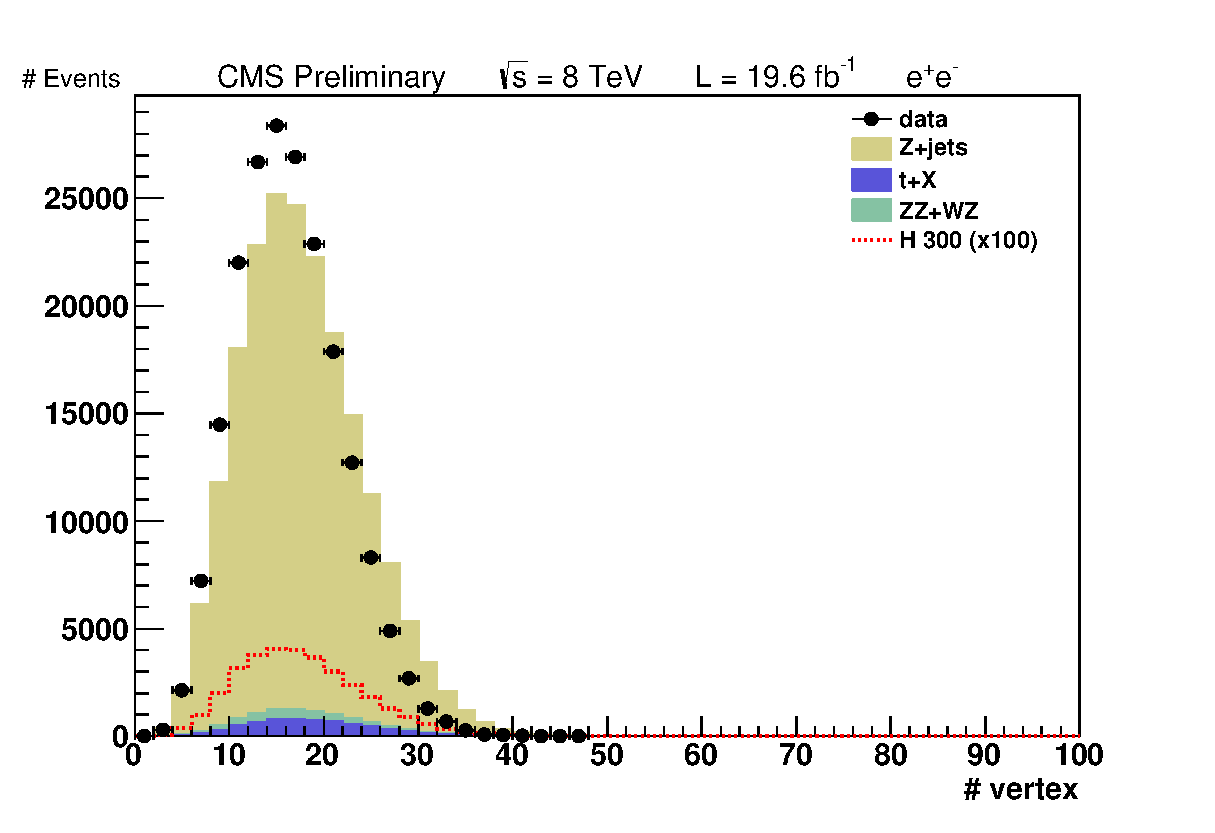
\includegraphics[width=0.49\textwidth]{Selection/before_el_nvtx.eps}
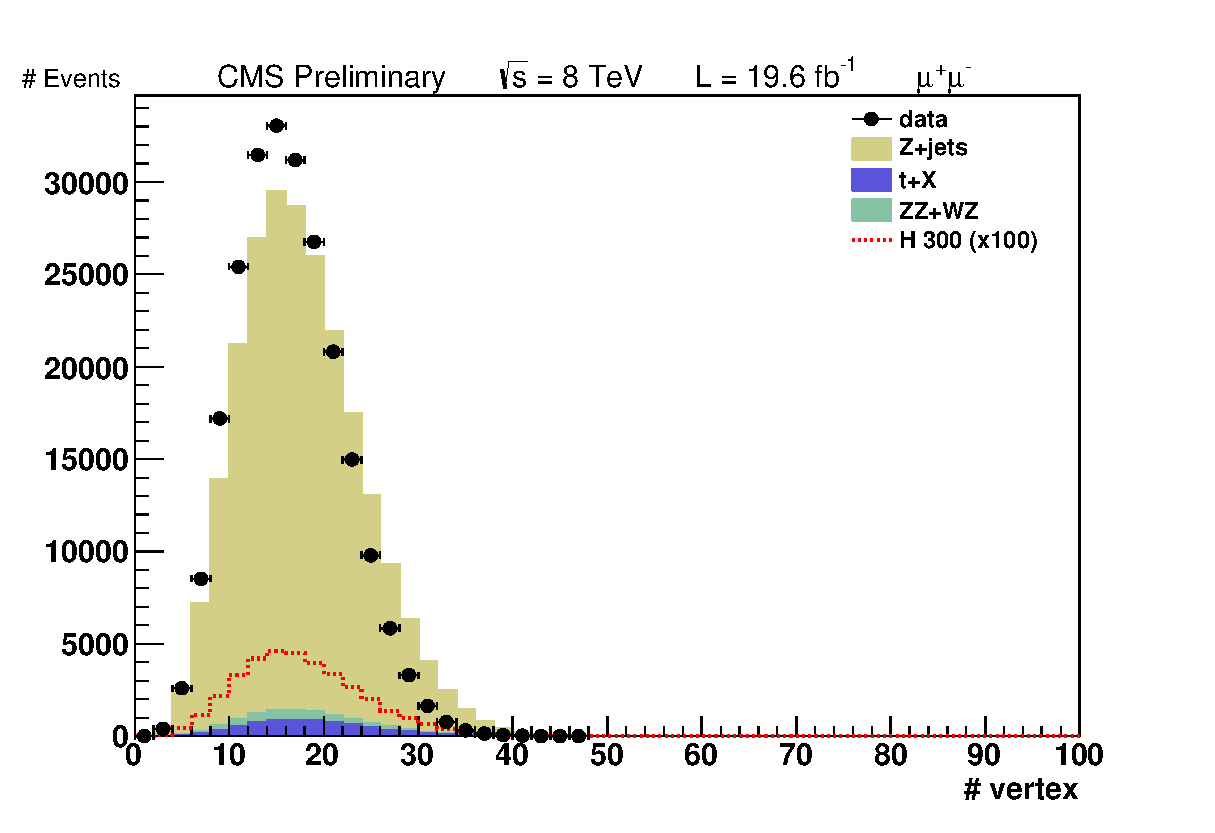
\includegraphics[width=0.49\textwidth]{Selection/before_mu_nvtx.eps}\\
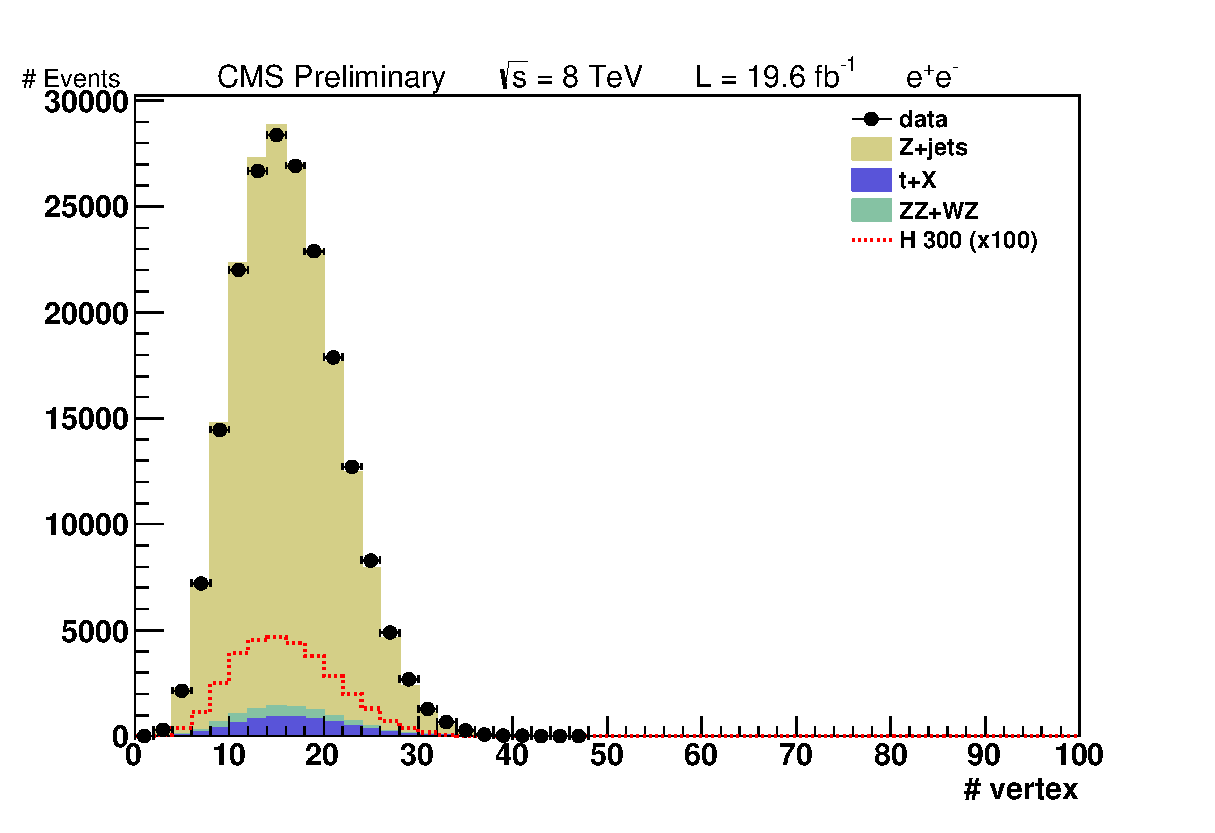
\includegraphics[width=0.49\textwidth]{Selection/after_el_nvtx.eps}
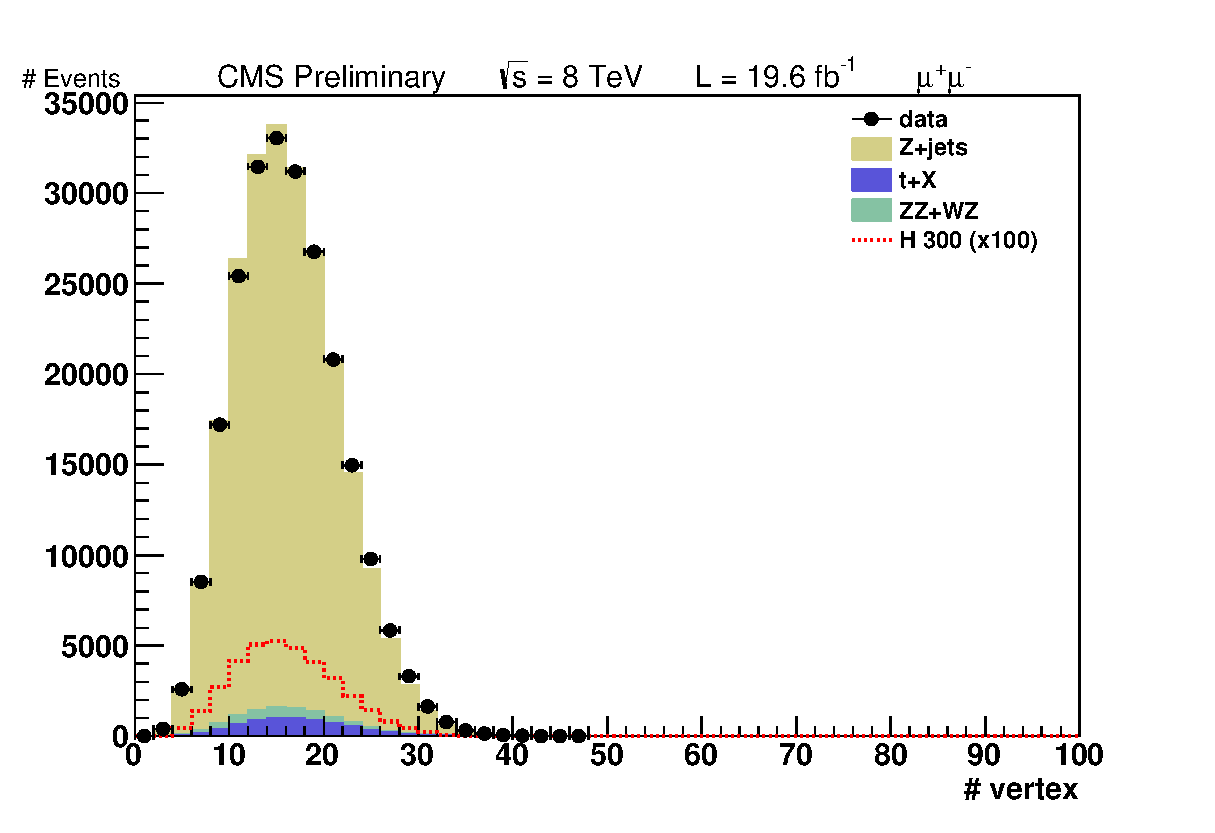
\includegraphics[width=0.49\textwidth]{Selection/after_mu_nvtx.eps}\\
\caption{Top Left: Number of interaction in the 2012 data and the simulated samples for electrons.  Top Right:  Number of interaction in the 2012 data and the simulated samples for muons. Bottom Left: Electron Monte Carlo pile-up corrected. Bottom Right: Muon Monte Carlo pile-up corrected.}
\label{fig:PileUp}
\end{figure}


%after_mu_nvtx.eps



\section{Preselection}
The Higgs boson signal events we are searching for have a signature of a lepton pair and a quark pair.  Both pairs will have an invariant mass that peaks around the Z boson mass.  $M_{lljj}$ is the invariant mass of the $\Plp \Plm \Pq \Paq$ system which corresponds to the hypothetical Higgs boson mass.  This is the main discriminating variable that we have to differentiate signal from background.

As mentioned above, particles are reconstructed from the measured detector interactions using the particle flow algorithm. We analyze events in the DoubleMu and DoubleElectron datasets. In each of these datasets, there is at least one un-prescaled trigger with looser requirements than the off-line selections. Only events which satisfy the lowest threshold un-prescaled trigger for the dataset are considered for the analysis. The trigger requirements are summarized in Table~\ref{triggers}.% More details on the trigger strategies for Higgs searches are available in~\cite{hlt}.

For muons in 2011, the {\tt HLT\_DoubleMu7} HLT was used and required that there were two muon candidates reconstructed at the HLT level.  Both of these had to have a transverse momentum larger than 7 GeV. As the luminosity of the LHC increased, this HLT was prescaled (only a fraction of the events passing were recorded) and we began to use {\tt HLT\_Mu13\_Mu8}.  This required the transverse momentum of one of the muons to be 13 GeV or larger and the other to be 8 GeV or larger.  Again this trigger was then prescaled because of increasing luminosity and the {\tt HLT\_Mu17\_Mu8} trigger was used for the final parts of 2011. Also the SingleMu dataset was added with the {\tt HLT\_IsoMu24} trigger to give a complete picture of the events. In 2012 only the {\tt HLT\_Mu17\_Mu8} trigger on the DoubleMuon dataset was used requiring one muon to have a transverse momentum above 17 GeV and another muon with transverse momentum above 8 GeV.  

Similar to the muon, HLT electrons are required to have one transverse momentum above 17 GeV and another electron with transverse momentum above 8 GeV.  In addition to this, there are a number of other requirements on isolation to reduce the number of fake electrons.

%%%%%%%%%%%%%%%%%%%%%%%%%%%%%%%%%%%%%%%%%%%%%%%%%
\begin{table*}[htb!]
\caption{ 
Event trigger requirements for data.
}
\label{triggers}
\vspace*{\medskipamount}
\begin{center}
\small
\begin{tabular}{|l l|}
\hline
\bf{Dataset} & \bf{2011 trigger requirement}   \\
\hline
DoubleMu & \tt{HLT\_DoubleMu7} \\
 & \tt{HLT\_Mu13\_Mu8} \\
 & \tt{HLT\_Mu17\_Mu8} \\ \hline
SingleMu & \tt{HLT\_IsoMu24} \\ \hline
DoubleElectron & \tt{HLT\_Ele17\_CaloIdL\_CaloIsoVL\_Ele8\_} \\ 
& \tt{CaloIdL\_CaloIsoVL} \\
 & \tt{HLT\_Ele17\_CaloIdT\_TrkIdVL\_CaloIsoVL\_TrkIsoVL\_} \\
 & \tt{Ele8\_CaloIdT\_TrkIdVL\_CaloIsoVL\_TrkIsoVL} \\ \hline
\bf{} & \bf{2012 trigger requirement}   \\
\hline
DoubleMu & \tt{HLT\_Mu17\_Mu8}\\
 & \tt{HLT\_Mu17\_TkMu8} \\ \hline
DoubleElectron & \tt{HLT\_Ele17\_CaloIdT\_TrkIdVL\_CaloIsoVL\_TrkIsoVL\_} \\ 
& \tt{Ele8\_CaloIdT\_TrkIdVL\_CaloIsoVL\_TrkIsoVL} \\
\hline
\end{tabular}
\end{center}
\end{table*}
%%%%%%%%%%%%%%%%%%%%%%%%%%%%%%%%%%%%%%%%%%%%%%%%%
Since the level of precision of the trigger emulation in simulation is not well known, no trigger is applied on MC samples. Instead, proper event weights are assigned to MC events according to the probabilities of lepton candidates to pass the trigger. The trigger efficiency tables for leptons satisfying the same identification criteria as in the analysis are computed in bins of ($pt$, $\eta$) from data using tag \& probe techniques~\cite{CMS-AN-2011-399}. 

\subsection{Lepton Selection}
$Z \rightarrow \Pem \Pep$ and $Z \rightarrow \Pgmm \Pgmp$ candidates are constructed from pairs of same-flavor, opposite-charge lepton candidates, which satisfy kinematic and identification criteria. Electron candidates are reconstructed with the GSF algorithm and in order to assure good electron reconstruction a cut is applied: the $\eta$ of the electron super-cluster must be inside the ECAL acceptance volume ($|\eta|<2.5$) but outside the ECAL barrel-endcap overlap region ($1.4442<|\eta|<1.566$). Muon candidates must have been reconstructed by both the GlobalMuon and the PF muon reconstruction algorithms and must satisfy the acceptance cut $|\eta|<2.4$.

Electron candidates must satisfy the standard ``Loose'' working point of the cut-based electron identification for 2012 analysis. The cuts are listed in Appendix~\ref{sec:datamcsf} and comprise proper electron identification requirements, an isolation cut, and conversion rejection criteria. Muon candidates must satisfy the standard ``Tight'' working point of the cut-based muon ID for 2012 analysis. The cuts are listed in Appendix~\ref{sec:datamcsf} and comprise proper muon identification requirements plus an isolation cut.

%%%%%%%%%%%%%%%%%%%%%%%%%%%%%%%%%%%%%%%%%%%%%%%%%
%\begin{table*}[htb]
%\caption{ 
%Electron ID requirements for the Loose ID working point.
%}
%\label{tab:electronid}
%\vspace*{\medskipamount}
%\begin{center}
%\small
%\begin{tabular}{|l|l|l|}
%\hline
%Variable & Barrel cut & Endcap cut  \\
%\hline
%$\Delta \eta_{trk, supercluster}$ & $<0.007$ & $<0.009$ \\
%$\Delta \phi_{trk, supercluster}$ & $<0.15$ & $<0.1$ \\
%$\sigma_{i\eta, i\eta}$ & $<0.01$ & $<0.03$ \\
%$H/E$ & $<0.12$ & $<0.10$ \\
%$d_{0}$ (wrt primary vertex) & $< 0.2 mm$ & $< 0.2 mm$ \\
%$d_z$ (wrt primary vertex) & $< 2 mm$ & $< 2 mm$ \\
%$|1/E - 1/p|$ & $< 0.05$ & $<0.05$ \\
%$I_{PF, \,\, corr}/p_T$ & $< 0.15$ & $<0.15$ \\
%Missing hits & $\le 1$ & $\le 1$ \\
%Conversion vertex fit prob.& $< 10^{-6}$ & $< 10^{-6}$ \\
%\hline
%\end{tabular}
%\end{center}
%\end{table*}
%%%%%%%%%%%%%%%%%%%%%%%%%%%%%%%%%%%%%%%%%%%%%%%%%
Given a lepton candidate, the PF isolation is defined as the sum of deposits (i.e. $p_T$ or $E_T$) of charged hadrons ($I_{ch}$), neutral hadrons ($I_{nh}$), and photons ($I_{ph}$), computed in a $\Delta R$ cone around the lepton direction. In order to assure independence of the isolation from the number of PU interactions, a corrected PF isolation definition is used as follows: 
\begin{equation} I_{PF, \,\, corr} = I_{ch}(PFnoPU) + max(I_{nh}+I_{ph}- \rho \cdot A_{eff} , 0) \end{equation}

In the above corrected definition, only deposits from charged hadrons not coming from PU vertexes ($I_{ch}(PFnoPU)$) are considered.  From these we subtract an overall PU energy contribution which is estimated as the average energy density in the event ($\rho$) multiplied by an effective area $A_{eff}$. This is strictly following the recommendations of egamma and muon POGs (Physics Object Group). The POGs are special groups within the CMS collaboration that define optimal methods of working with physics objects. The isolation cone for electrons is defined as $\Delta R < 0.3$, while for muons is defined as $\Delta R < 0.4$. The proper $A_{eff}$ values are provided by the POGs in bins of lepton $\eta$. A cut is applied on the relative PF isolation ($I_{PF, \,\, corr} / p_T$) as reported in Appendix~\ref{sec:datamcsf}.
%%%%%%%%%%%%%%%%%%%%%%%%%%%%%%%%
%\begin{table*}[htb!]
%\caption{ 
%Muon ID requirements for the Tight ID working point.
%}
%\label{tab:muonid}
%\vspace*{\medskipamount}
%\begin{center}
%\small
%\begin{tabular}{|l|l|}
%\hline
%Variable & Cut  \\
%\hline
%isGlobalMuon & True \\
%isPFMuon & True \\
%$\chi^2 / ndof$ (global fit) & $<10$ \\
%Muon chamber hits in global fit & $>0$ \\
%Muon stations with muon segments & $>1$ \\
%$d_{xy}$ (from tracker, wrt primary vertex) & $< 2 mm$  \\
%$d_z$ (from tracker, wrt primary vertex) & $< 5 mm$  \\
%Valid pixel hits (tracker track) & $> 0$ \\
%Tracker layers with hits & $>5$ \\
%$I_{PF, \,\, corr}/p_T$ & $< 0.12$ \\
%\hline
%\end{tabular}
%\end{center}
%\end{table*}
%%%%%%%%%%%%%%%%%%%%%%%%%%%%%%%%%%%%%%%%%%%%%%%%%




$Z \rightarrow ee $ and $Z \rightarrow \mu\mu$ candidates are constructed from pairs of opposite-charge leptons. The leading lepton of the pair must have $p_T > 40 GeV$,
while the next-to-leading lepton must have $p_T > 20 GeV$. The invariant mass of the pair must be $ 70 < m_{\ell \ell} < 110 GeV $. The di-lepton invariant mass for the selected $Z \rightarrow \ell \ell$ candidates is shown in Fig.~\ref{fig:m_dilepton}.  
%%%%%%%%%%%%%%%%%%%%%%%
\begin{figure}[htb!]
\begin{center}
\centerline{
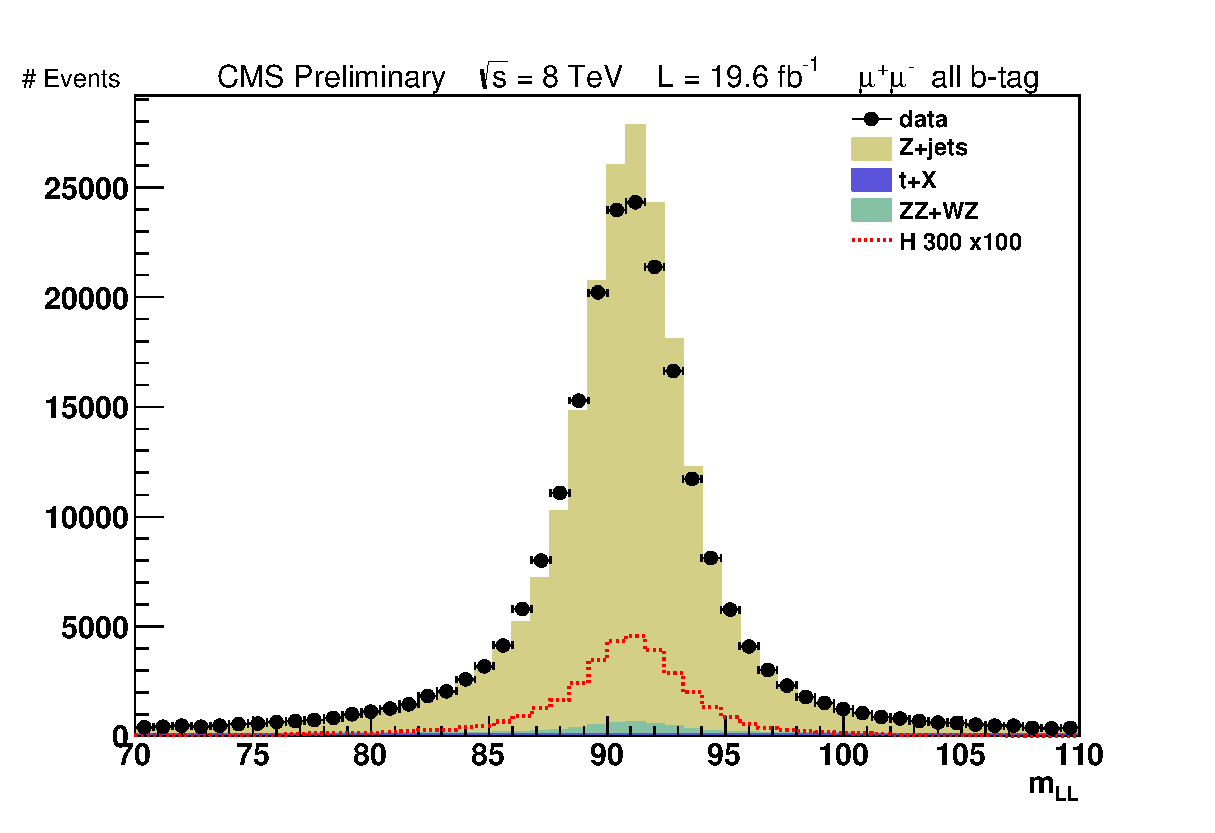
\includegraphics[width=0.45\textwidth]{presentation/defense/images/preselection/mu/mLL.eps}
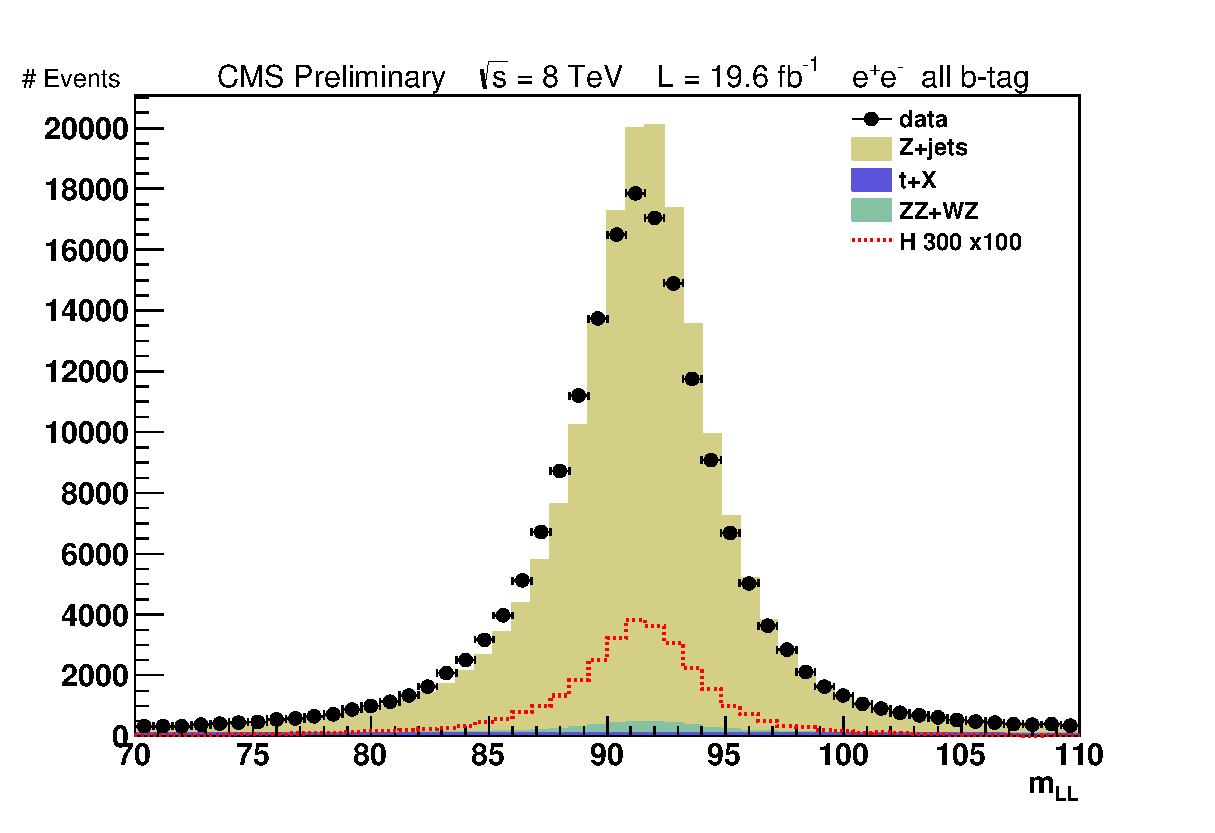
\includegraphics[width=0.45\textwidth]{presentation/defense/images/preselection/el/mLL.eps}
%\includegraphics[width=0.45\textwidth]{plots//tmva_massZll.eps}
}
\caption{
Di-lepton invariant mass in data and MC of $Z \rightarrow \ell \ell$ candidates after lepton selection. Left: Muon channel. Right: Electron channel. The selection described in preselection is applied except for the cut on $m_{jj}$.
}
\label{fig:m_dilepton}
\end{center}
\end{figure}
%%%%%%%%%%%%%%%%%%%%%%%

\subsection{Jet Selection}
\label{sec:jetsel}
The PF jets are reconstructed with the anti-k$_{T}$ algorithm ~\cite{antikt} with radius parameter set to $R=0.5$. Jets are required to be inside the tracker acceptance ($|\eta|<2.4$) thus allowing high reconstruction efficiency and precise energy measurements using PF techniques. Jet-energy corrections are applied to data and Monte Carlo~\cite{CMS-PAS-JME-10-010}. Correction for PU energy is applied at the first level, by using the Fastjet algorithm~\cite{FastJet}. In order to remove jets which originate from PU interactions, only jets with $\beta \ge 0.2$ are selected, where $\beta$ is defined as the sum of transverse momenta of all charged particles in the jet coming from the primary vertex, normalized to the total sum of transverse momenta of all charged particles in the jet. The $\beta$ distribution and efficiency can be seen in Figure~\ref{fig:beta}~\cite{2l2q115}. $Z \rightarrow q\overline{q} $ candidates are reconstructed from jet-jet pairs. In order to reject fake candidates made by low-$p_T$ jets from QCD background, both jets of the pair must have $p_T > 30 GeV$.


\begin{figure}[htb]
\begin{center}
\centerline{
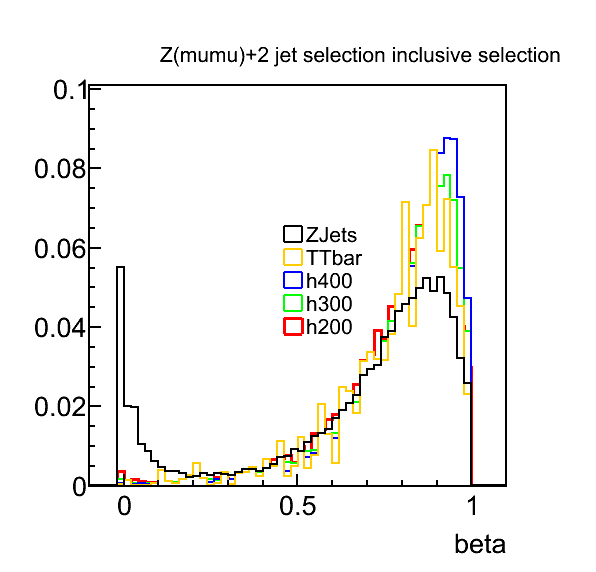
\includegraphics[width=0.50\textwidth]{Selection/beta_Zmm.png}
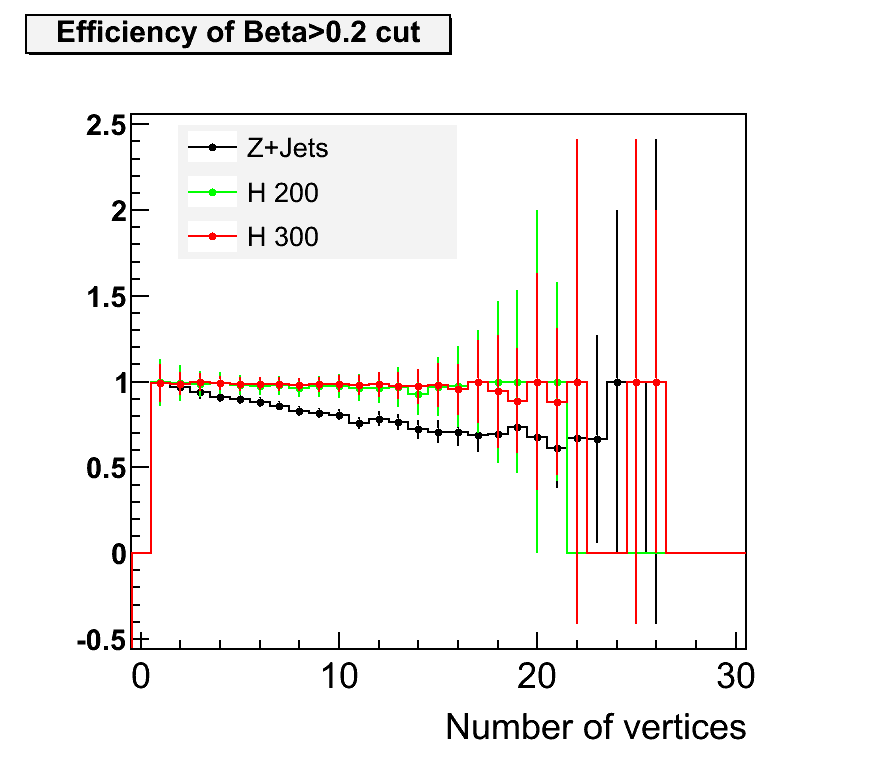
\includegraphics[width=0.50\textwidth]{Selection/beta_eff.png}
%\includegraphics[width=0.45\textwidth]{plots//tmva_massZjj.eps}
}
\caption{
$\beta$ fraction of the total transverse momentum of charged particles in a jet that is computed from particles pointing to the primary interaction for different background and signal samples (left) and efficiency of a cut in $\beta <$ 0.2 for signal with Higgs mass of 200 GeV and 300 GeV and Z+Jets background, as a function of the number of reconstructed vertices in an event(right).~\cite{2l2q115}
}
\label{fig:beta}
\end{center}
\end{figure}


A loose jets identification is applied to the jets to remove fake jets that arise from calorimeter noise.  These requirements are summarized in table~\ref{tab:jetcuts}.  In the analysis a cut around the Z mass is done for 75 $< m_{jj} <$ 105 GeV to help control the Z+jets background.  The $m_{jj}$ distributions for electron and muon channels can be seen in Figure~\ref{fig:mjj}.
%%%%%%%%%%%%%%%%%%%%%%%%%%%%%%%%
\begin{table*}[htb!]
\caption{ 
Jet cuts to remove fakes.
}
\label{tab:jetcuts}
\vspace*{\medskipamount}
\begin{center}
\small
\begin{tabular}{|l|l|}
\hline
Variable & Cuts\\
\hline
fraction of energy due to neutral hadron & $<$ 0.99 \\
fraction of energy due to neutral EM deposits & $<$ 0.99 \\
number of constituents & $>$ 1 \\
number of charged hadrons candidates & $>$ 0 \\
fraction of energy due to charged hadron candidates & $>$ 0 \\
fraction of energy due to charged EM deposits & $<$ 0.99 \\
$\beta$ & $>=$ 0.2  \\
\hline
\end{tabular}
\end{center}
\end{table*}
%%%%%%%%%%%%%%%%%%%%%%%%%%%%%%%%%%%%%%%%%%%%%%%%%

%%%%%%%%%%%%%%%%%%%%%%%
\begin{figure}[htb]
\begin{center}
\centerline{
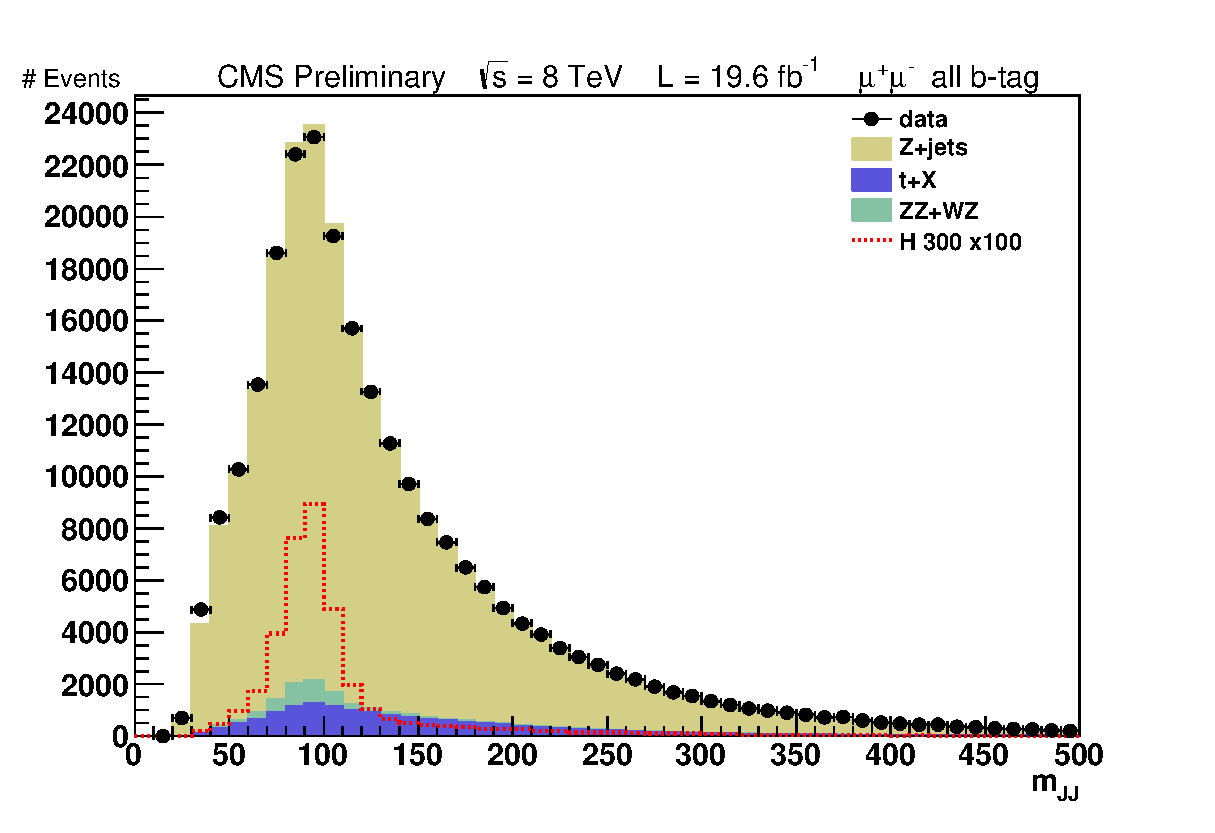
\includegraphics[width=0.45\textwidth]{presentation/defense/images/preselection/mu/mJJ.eps}
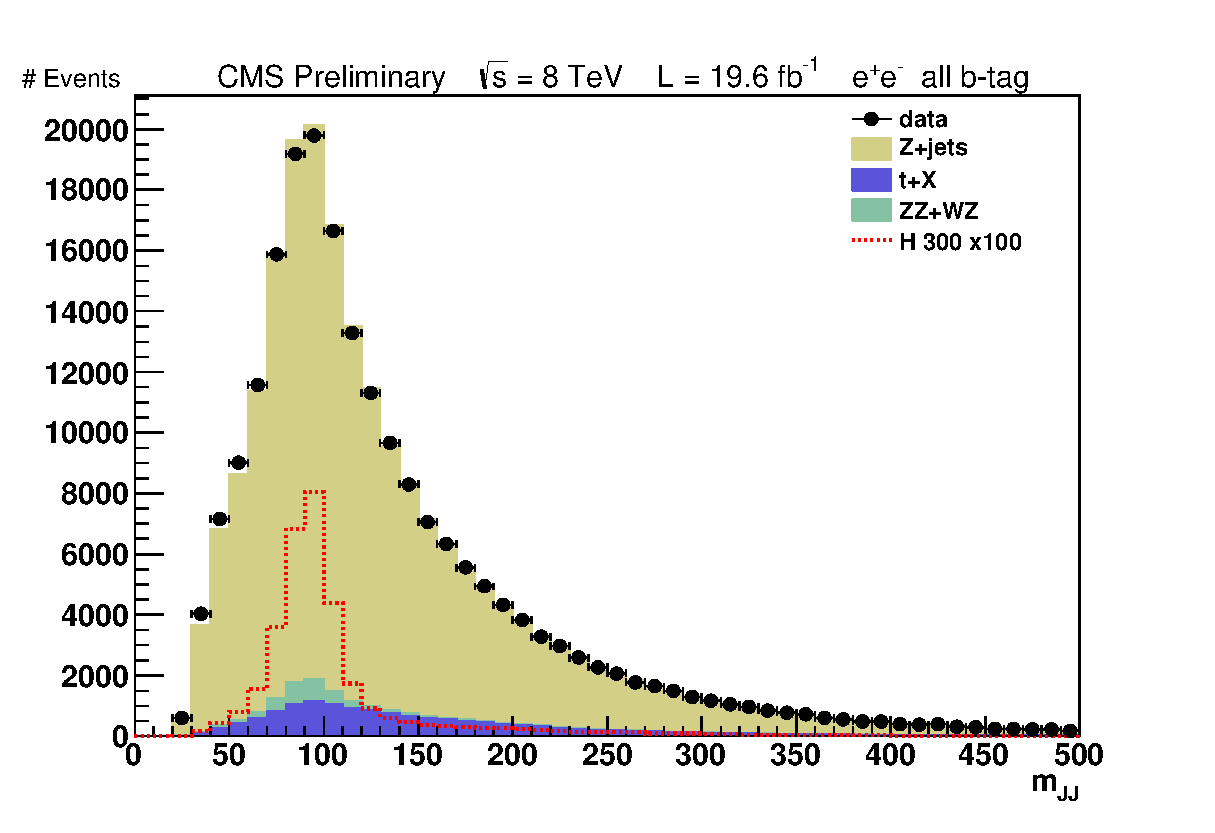
\includegraphics[width=0.45\textwidth]{presentation/defense/images/preselection/el/mJJ.eps}
%\includegraphics[width=0.45\textwidth]{plots//tmva_massZjj.eps}
}
\caption{
Di-jet invariant mass in data and MC for $\ell \ell jj$ candidates which have passed the preselection. Left: Muon channel. Right: Electron channel.
}
\label{fig:mjj}
\end{center}
\end{figure}
%%%%%%%%%%%%%%%%%%%%%%%

\subsection{B-tagging of jets}
\label{subsec:btaggingofjets}
Due to the relatively large branching fraction of the $Z$-bosons decaying into a pair of bottom-anti-bottom quarks, compared to the abundance of light-quark or gluon jets in $Z$+jets background events, we use a b-tagging algorithm in order to identify jets originating from heavy-flavor quarks. However, no selection of candidates based on b-probabilities is employed in the analysis. Instead, the b-tagging information is used to classify $\ell \ell jj$ candidates into three categories, each one characterized by a certain signal-to-background ratios, and an optimized selection is applied on candidates belonging to different categories~\cite{CMS-AN-2011-399}. This exploits as much information as possible from the data increasing the analysis sensitivity.

With Z+jets as the main background, this is primarily described by a Z boson that decays leptonically in conjunction with the production of high $p_T$ jets. These jets are primarily produced from gluon radiation as well as light quark hadronization.  These light quarks come from the fact that u and d quarks make up the valence partons of the proton. One of the main differences for signal and background is that the signal will not contain gluons, and relative to the background, will have a large contribution of heavy flavor quarks.

We are using the CMS Jet Probability (JP) tagging algorithm for b-jets~\cite{CMS-PAS-BTV-11-004}.  This uses the relative long lifetime of bottom hadrons with the tracks from the PF algorithms to estimate if the jet came from the primary vertex.  If this probably is low then the jet has a larger probability of being a b-jet.  The good performance of this b-jet identification is possible because of the the precision tracking of charged particles and lepton identification at CMS.

The output of the JP algorithm is a discriminator for each jet in the event.  This distribution for data and simulated events can be seen in Figure~\ref{fig:JP} for electrons and muons.  To discriminate between jets that are coming from heavy flavor quarks (c,b) with those coming from light flavor quarks (d,u,s) we use two separate values from the JP algorithm.  The first point, called the loose working point (L), is set at a value of the output of the JP algorithm equal to 0.0275. This working point corresponds to a mis-identification probability that the jet is a light flavored jet of 10\%.  The medium working point (M) has a value of 0.545 and has a mis-identification probability of 1\%.  These are abbreviated as JPL and JPM for the loose and medium working points respectively.


A summary of all the selection can be found in section~\ref{sec:summaryofselectionrequirements}.
%Details of the b-tagging algorithm are described in section%~\ref{sec:btag} and candidates 
%categories are defined in section%~\ref{ssec:classification}


%%%%%%%%%%%%%%%%%%%%%%%
\begin{figure}[htb]
\begin{center}
\centerline{
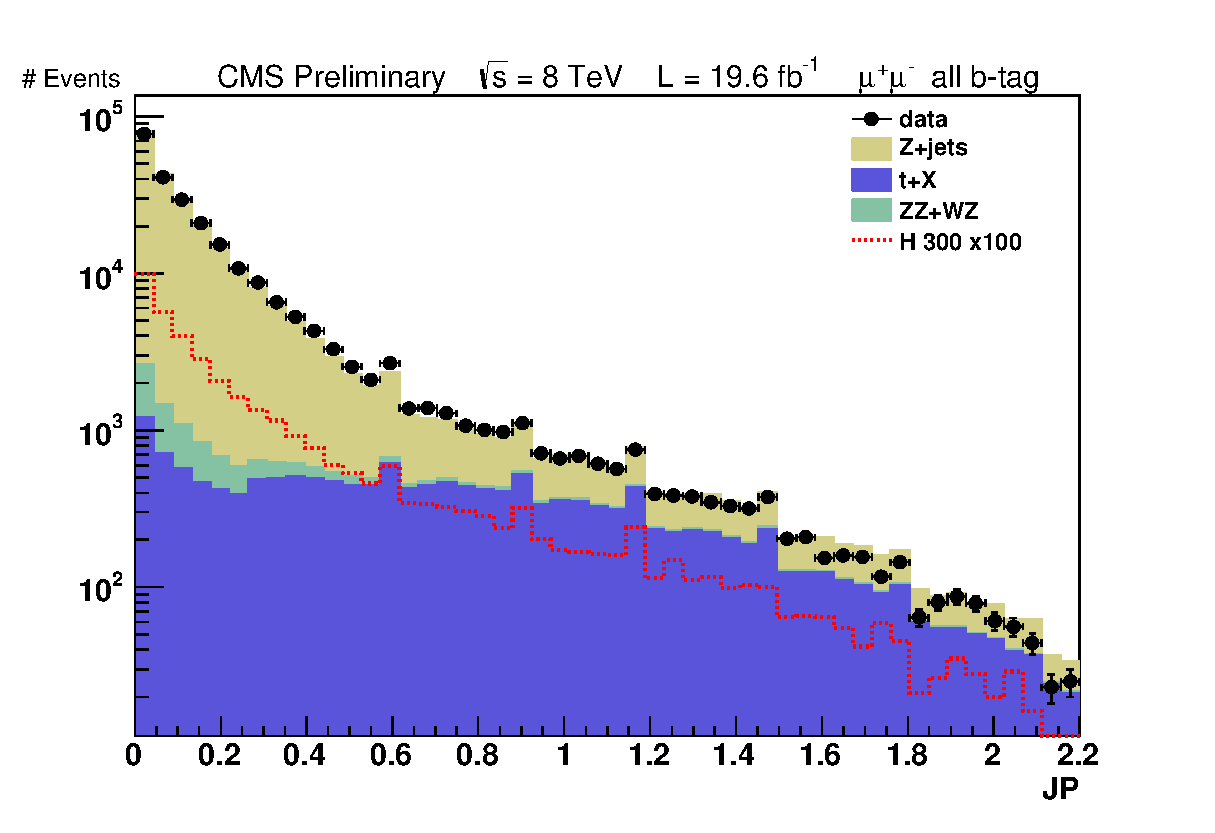
\includegraphics[width=0.49\textwidth]{presentation/defense/images/preselection/mu/j0jp_log.eps}
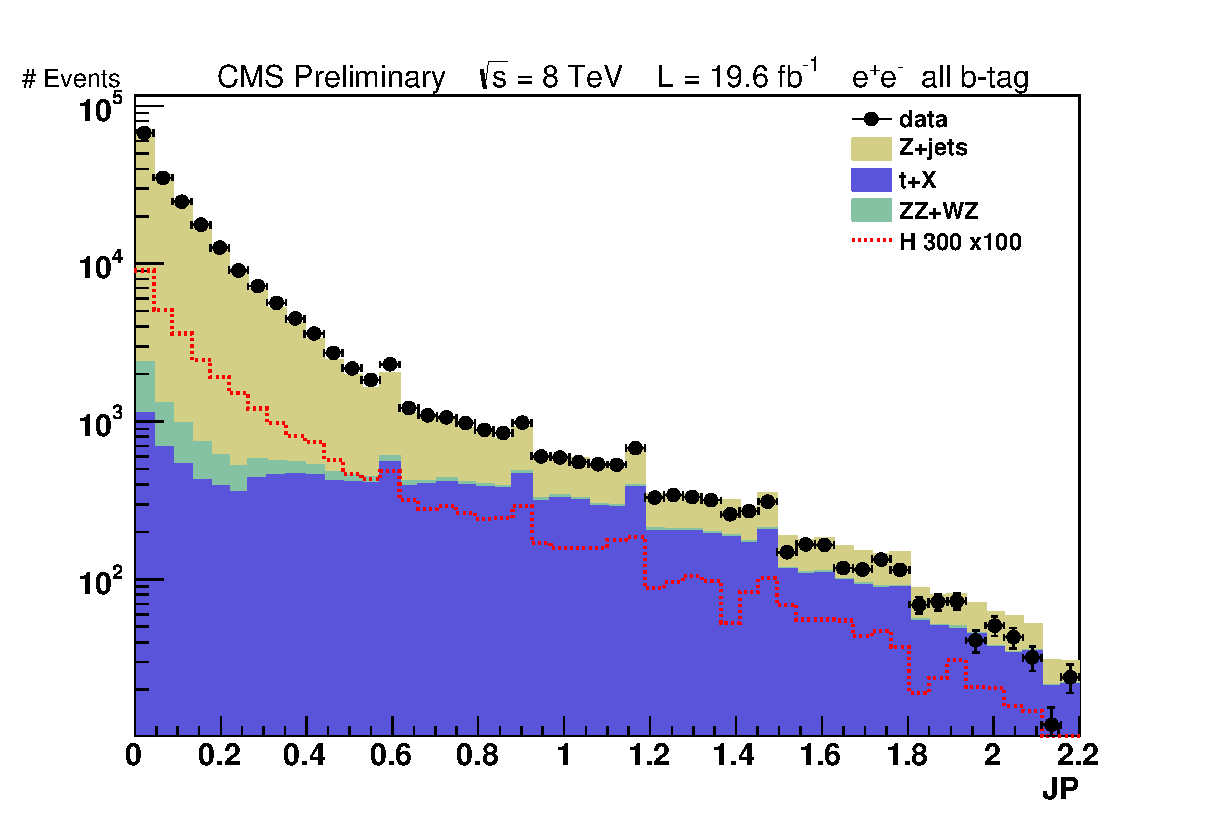
\includegraphics[width=0.49\textwidth]{presentation/defense/images/preselection/el/j0jp_log.eps}
%\includegraphics[width=0.45\textwidth]{plots//tmva_massZjj.eps}
}
\caption{
Distribution of the jet probability (JP) discriminator that is used for b-tagging.  Right: Muons. Left: Electrons. The peaks in the distribution come from calculating the jet probability non-continuously in $\eta$ bins. This phenomenon is well understood and expected.
}
\label{fig:JP}
\end{center}
\end{figure}
%%%%%%%%%%%%%%%%%%%%%%%


\subsection{Higgs candidates}
\label{sec:reco}
All the leptons and jets that satisfy the above requirements are combined to form both leptonic and hadronic Z bosons.  For each event, the dilepton and dijet pairs are combined to create $\ell \ell jj$ events or Higgs candidates. A $\Delta R > 0.5$ cut is applied between each lepton and jet within a candidate in order to avoid double counting of the same object reconstructed in different collections (for instance leptons inside a jet). An example event with a Higgs boson candidate decaying to two muons and two jets can be seen in Figure~\ref{fig:event_display}~\cite{CMS-PAS-HIG-12-024}. In the following sections, the previous requirements on Higgs candidates and their constituent particles will be referred to as preselection.

%%%%%%%%%%%%%%%%%%%%%%%
\begin{figure}[htb]
\begin{center}
\centerline{
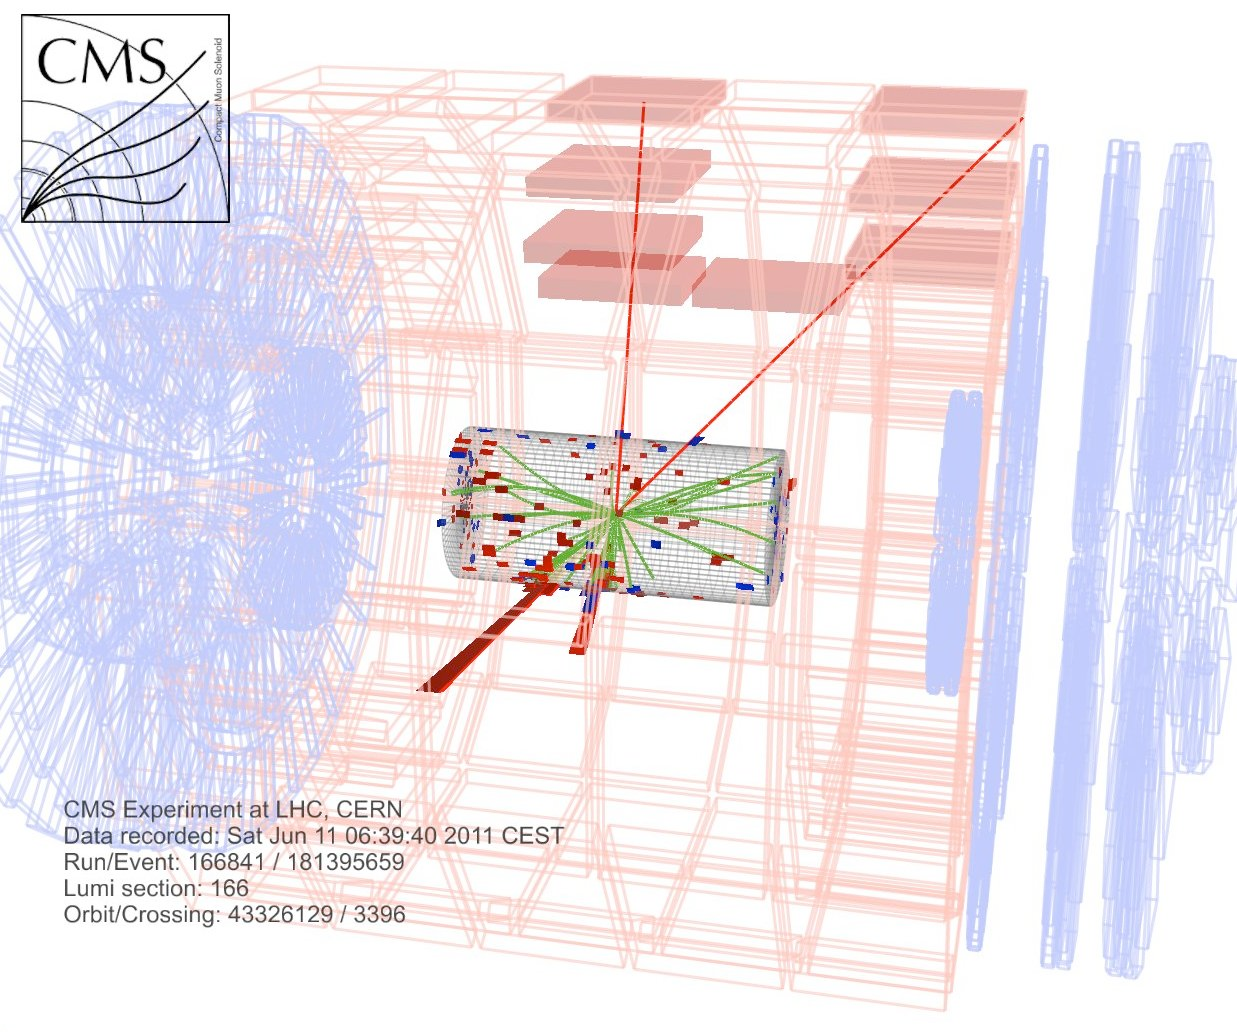
\includegraphics[width=0.85\textwidth]{Selection/eventDisplay7TeV.png}
%\includegraphics[width=0.45\textwidth]{plots//tmva_massZjj.eps}
}
\caption{
An event display of a Higgs event candidate decaying to two muons and two jets.~\cite{CMS-PAS-HIG-12-024}
}
\label{fig:event_display}
\end{center}
\end{figure}
%%%%%%%%%%%%%%%%%%%%%%%

